\chapter{Introduction \& Motivation}
\label{chapter:introduction}
%
\epigraph{\textit{I wish to God these calculations had been executed by steam.}}{Charles Babbage}
The advent of the modern digital computer, as formalised by Alan Turing,\cite{Turing1937} ignited the field of computational physics, aided by preexisting theoretical formulations of algorithms. Starting from the first experiments with Monte Carlo (MC) simulations in the 1930s by Fermi and the formulation of the Markov-Chain Monte Carlo (MCMC) technique by Ulam in the 1940s, von Neumann programmed the 18,000 vacuum-tube Electronic Numerical Integrator and Computer (ENIAC) computer to investigate neutron diffusion in fissionable materials.\cite{metropolis1987beginning} This success paved the way for the integration of Newton's equations of motion to compute the time evolution of a many-body system.\\

Consider being Marian Adam Rejewski, a Polish mathematician and cryptologist in 1932, almost
seven years before the beginning of World War II. It was known at the time that the Germans
were using a machine called \textit{Enigma I} to send secret messages, but no one knew what
the machine looked like nor how it worked. Based on a handful of intercepted encrypted
messages and pictures of the operating instructions obtained by Polish intelligence,
he derived a set of permutation equations that allowed him the reverse-engineer the machine
\cite{Turing2018XBroken}. The cryptologic achievements of Rejewski and colleagues
Jerzy R\'o\.zycki and Henryk Zygalski are considered the some of the greatest feats in
reverse-engineering of the 20th century.

\begin{Figure}
    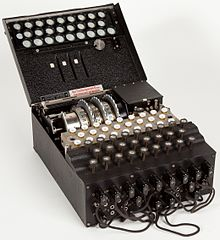
\includegraphics[width=40mm]{figures/enigma.jpg}
    \caption{\textit{Enigma I} reverse engineered by Marian Adam Rejewski}
    \label{fig:enigma}
\end{Figure}
\noindent

Today we are getting ever closer to reverse-engineering the cell.
The fields of synthetic and systems biology are beginning resemble engineering disciplines;
genetic engineering is becoming more precise, high-throughput in vitro experiments are performed
by robots and measurements of many desired observables can be obtained with high spatio-temporal resolution.
Advances in micro-fabrication \cite{Shafiee2017TissueMedicine} and in-vitro reconstitutive methods \cite{Gopfrich2018MasteringCells} have allowed biologists isolate pathways and mechanisms to a level of
mathematical and computational tractability \cite{Sharpe2017ComputerTomorrow.}. This section
outlines the scientific paradigms in these fields, their methods and limitations, and finally what this
thesis will attempt to contribute.

\section{Bottom-up and Top-down Biology}

Fortunately for biologists copies of the target of their reverse-engineering attempts are
available all around us. Less fortunate is the fact that most attempts at deconstructing
the cell end in loss of function and destruction of the individual components. This
restriction motivates system biologists to manipulate environmental signals \textit{in vivo}
and build mechanistic models from correlations between signals and responses \cite{Triantafillou2017PredictingCells}.
Models focus on relationships between macroscopic variables where the underlying
mechanisms are not known.
\\\\
\textit{In vitro} reconstitutive methods aim to isolate minimal mechanisms from the
complexity of the whole organism in order to unpick the relative importance of
microscopic details \cite{Gopfrich2018MasteringCells}.
In situations where purified proteins and crystal structures
are available these methods can quite accurately characterise the kinetics of
proteins. Relating these parameters to the \textit{in vivo} context however may
not be relevant, as too much of the complexity may have been stripped away. 
\\\\
From a theoretical modelling perspective, it is important to choose a time-scale
and space-scale that is relevant to the problem. If one is interested in tissue
dynamics, attempting to model DNA conformations within each cell will render the
problem intractable. As George Booth aptly put \textit{``most models are wrong but
some are useful"} so the role of theoretical descriptions in these settings is not
necessarily to describe the way reality \textit{is} but serve as tools to bridge
the non-intuitive gap between bottom-up and top-down approaches. Where intuition
fails is where the \textit{in silico} hypothesis testing playground becomes most
valuable \cite{Sharpe2017ComputerTomorrow.}.

\begin{Figure}
    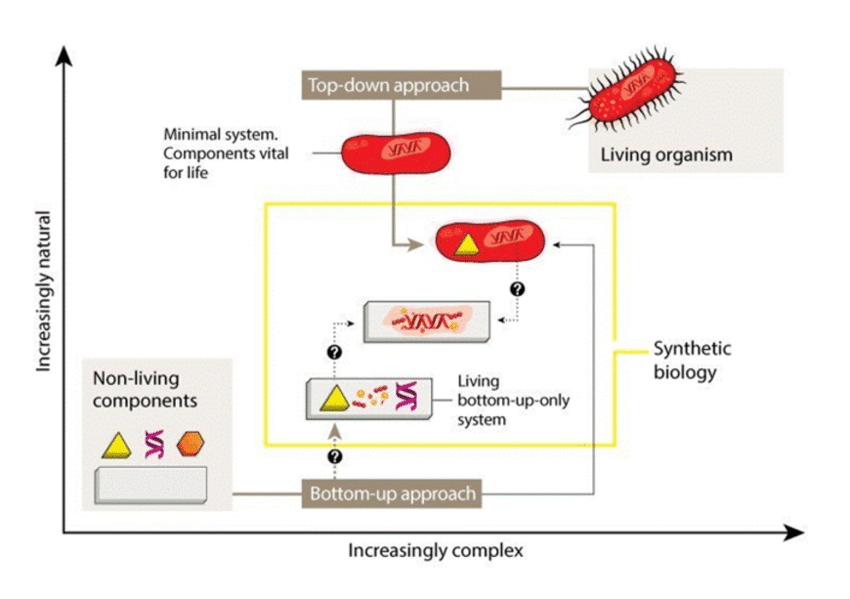
\includegraphics[width=80mm]{figures/top-down-bottom-up.png}
    \caption{Top-down and bottom-up modelling methods}
    \label{fig:tdbu}
\end{Figure}

\section{Design, Build, Test, Learn}
Systems and synthetic biology have historically made progress through a process
of brute force trial and error. This usually involves the interaction of many
custom-made parts that are iteratively optimised by human intervention. A trend
first observed in the 1980s known as \textit{Eroom's law} reveals that discoveries
in biotechnology are becoming slower and more expensive over time, despite
improvements in technology \cite{Scannell2012DiagnosingEfficiency}.
This problem is compounded by the ongoing reproduciblility crisis \cite{Ioannidis2005WhyFalse.}.
In the effort to transform methods used in academia and industry to become more
systematic and predictable, a standard for the Design--Build--Test--Learn cycle
has emerged -- showin in figure \ref{fig:dbtl}.
\\\\
This workflow has now been established as a paradigm with some aspects that have
been automated by liquid handling robots, bioreactor environments and image processing
pipelines. However, humans in the loop and custom moving parts still persist. The challenge
in automating these processes lies in defining a programming language that has a
sufficiently high level of abstraction for transparent implementation
while allowing for low-level customisation \cite{Abate2018ExperimentalSemantics}.

\begin{Figure}
    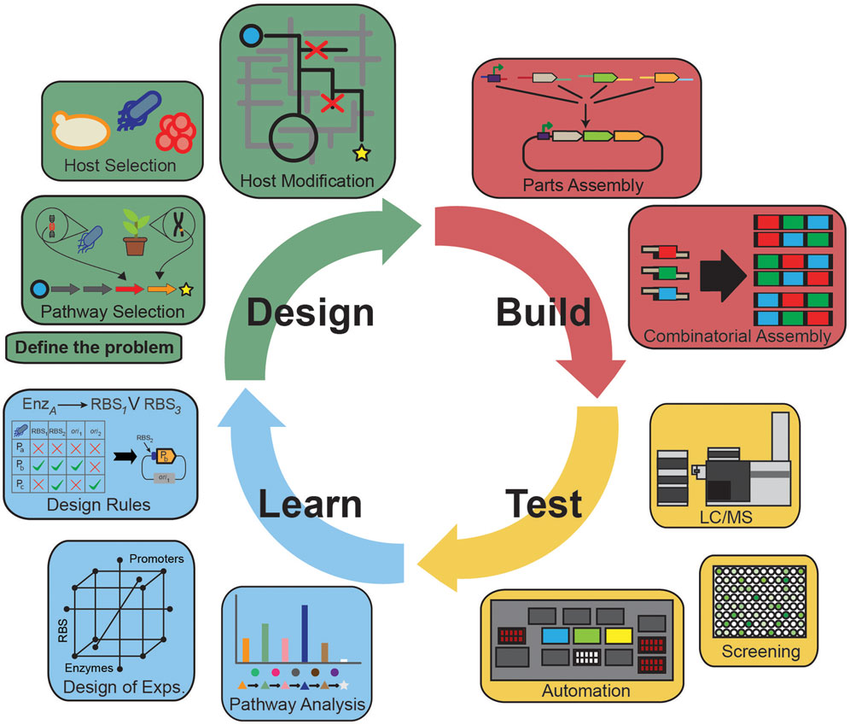
\includegraphics[width=60mm]{figures/dbtl.png}
    \caption{Design-Build-Test-Learn cycle from synthetic biology}
    \label{fig:dbtl}
\end{Figure}
\noindent
This thesis will focus on modelling and inference using systems of differential
and partial differential equations, which fits into the Design--Learn part of
the cycle. Differential equations occupy a small subset of possible modelling tools,
however they are amongst the most popular due to their ease of use formulation
and simulation. This ease of access creates a zoo of models in literature making
it difficult to identify the key ingredients that distinguish different models.
Furthermore the relationship between multiple plausible \textit{and} in-plausible hypotheses
is rarely investigated. This motivates desire for an automated Design--Learn pipeline --
outlined in Section \ref{section:design-learn} -- which can generate and catalogue models
in a transparent manner while producing insights for the Build stage.
This pipeline is applied in an experiment-theory collaboration described in
Chapter \ref{chapter:double-exclusive}.

\section{State of the Art}
\label{section:geometry}
\subsection{Inference of Differential Equations}
Following the initial literature on smooth and match estimators
\cite{Gugushvili2012Smoothing} -- which overcome the bottleneck
having to integrate a proposed hypothesis for every parameter update --
a plethora of methods for the inference of differential equations
became available \cite{Brunton2016SparseSINDYc,GorbachScalableSystems}.
The essence of these methods is to estimate the derivatives of the
data rather than integrate the model and simultaneously estimate 
the qualitative and quantitative behaviours. In most biological
experiments batch-to-batch variations decrease the certainty
with which it is possible to quantify a behaviour. Whether or not
a parameter is identifiable, reduntant or sloppy have become
key questions in biology \cite{Chis2016OnIdentifiability,
Gabor2017ParameterBiosystems,Villaverde2016StructuralModels}.

\subsection{Model Reduction and Classification}
Sloppiness and sensitivity anaylsis have been extensively used in the
search for reduced models. Linear
mappings between models that preserve stoichiometry and reactant structure were
investigated \cite{Cardelli2014MorphismsFunction,Cardelli2017MaximalSystems} and
computational tools based on partition-refinement were released
\cite{Cardelli2017ERODE:Equations}. Structural similarity between reaction
networks can be revealed by such mappings, elucidating the functional aspects of
complex networks in terms of simpler networks. The aim of the Design--Learn
pipeline is to extend this framework to nonlinear mappings with an emphasis on
geometry rather than kinetics. Most inference techniques attempt to match
geometry and kinetics simultaneously in an attempt to obtain a quantitative
model. This thesis emphasises that geometry alone should be prioritised in
order to obtain qualitatively equivalent models. Furthermore recent
results in pattern formation theory \cite{Halatek2018} do not depend
on kinetics at all, only geometry.

\section{Design--Learn Pipeline}
\label{section:design-learn}

This section outlines the proposal for a design--learn pipeline for
the purposes of model reduction and system design. Suppose experimental
collaborators have provided us with time-course gene expression data $\mathcal{D}$,
which could be taken via time-lapse microscopy of cells growing on microfluidic plates,
optical density measurements from microtiter plate assays or temporal snapshots of
flow cytometry measruements. On the other hand one may want to specify a behaviour
$\mathcal{H}$ which may have not yet been observed. This would be specified with
top-down constraints, i.e. there exist oscillations of a fixed frequency or
a region of bistability.

\subsection{Experimental Design Loop}
\label{section:experimental-design}

The experimentalists may want to know whether the data collected could
result in a model of predictive power without mechanistic knowledge
of the underlying biochemistry. Moreover it would be desirable gain insights
in parameter regimes in the vicinity of observations, without having to
wait for the theorists to produce a refined model. Such real-time insights
would guide data collection protocols, optimising the amount of information
gained while keeping the number of experiments performed to a minimum. Often
data is noisy and at worst case contradictory; these issues must also be exposed.

\begin{Figure}
    \begin{tikzpicture}[node distance=2cm]

        \node (nonparametric) [process, minimum width=5cm] {non-parametric inference};
        \node (data) [io, right of=nonparametric, xshift=1cm, yshift=2cm] {observations $\mathcal{D}$};

        \node (field) [decision, below of=nonparametric] {field $\Vector{f}$};
        \node (pred) [io, right of=field,  xshift=2cm] {predictions};

        \draw [arrow] (data) |- (nonparametric);
        \draw [arrow] (nonparametric) -- (field);
        
        \draw [arrow] (field) -- (pred);
        \draw [arrow,color=BurntOrange] (pred) -- +(0,3.5);

    \end{tikzpicture}
    \caption{Workflow loop for optimal experimental design, without mechanistic model}
    \label{fig:experimental-design}
\end{Figure}
\noindent
Figure \ref{fig:experimental-design} outlines the workflow for optimal experimental design.
The term \textit{non-parametric} defines the procedures that have prioritised  
functional generality and flexibility over mechanistic insights gained from the values
of the parameters and shapes of the mathematical forms. Neural networks and Gaussian process
regressors are examples of non-parametric estimation procedures, which produce an estimate
of the field $\Vector{f}$ that predicts gene expression rates at given expression levels.
Based on these predictions, the experimentalist may proceed to collect data in the most
informative parameter regions, which would in turn more accurately estimate $\Vector{f}$.

\subsection{Hypothesis Scoring and Model Refinement Loop}
\label{section:refinement}
Often predictions from field $\Vector{f}$ are not enough. Models constructed
with feasible biophysical assumptions $\Vector{h}(\Vector{\theta})$ have the potential
to extrapolate predictions and give concrete biophysical meanings to each parameter $\Vector{\theta}$.
This way the experimentalist knows exactly which modification to the system they must
make in order to achieve a desired behaviour. More often than not it is also unclear
whether the model and its assumptions are reasonable, which brings us to the desire
to score our hypotheses. For increased
accuracy and efficiency \cite{Meeds2019EfficientSystems} the mechanistic model
$\Vector{h}(\Vector{\theta})$ is inferred against non-parametric estimate $\Vector{f}$
rather than the data $\mathcal{D}$ directly. Furthermore as discussed in Section
\ref{section:geometry} the aim is to optimise geometry rather than kinetics.
Alternatively one may construct $\Vector{h}(\Vector{\theta})$ to cover a whole class
of models, such as those that satisfy mass-action. The expectation is that most of the
parameters would be zero but some would be informative. One can obtain a distribution
of optimal parameters $\rho(\Vector{\theta})$ by running multiple optimisations. From
this distribution one may construct alternative hypotheses and update $\Vector{h}(\Vector{\theta})$.
By iterating this procedure one would identify the minimal model within the model class that
explains the data. This process is known as model refinement or reduction.

\begin{Figure}
    \begin{tikzpicture}[node distance=2cm]

        \node (field) [decision] {field $\Vector{f}$};
        \node (hypothesis) [io, left of=field,  xshift=-2cm] {hypothesis $\Vector{h}(\Vector{\theta})$};
        \node (parametric) [process, below of=field, minimum width=5cm] {geometric inference};
        
        \node (params) [io, below of=parametric] {parameter distribution $\rho(\Vector{\theta})$};
        \node (score) [io, right of=params, xshift=4cm] {score};
        \node (decomp) [process, below of=params, minimum width=5cm] {clustering and decomposition};
        \node (models) [io, left of=decomp, xshift=-3cm] {models};

        \draw [arrow] (field) -- (parametric);
        \draw [arrow] (hypothesis) |- (parametric);
        \draw [arrow] (parametric) -- (params);
        
        \draw [arrow] (params) -- (decomp);
        \draw [arrow] (params) -- (score);
        \draw [arrow] (decomp) -- (models);
        \draw [arrow,color=ForestGreen] (models) -- +(0,5.5);

    \end{tikzpicture}
    \caption{Overview of hypothesis scoring pipeline and model refinement loop}
    \label{fig:non-parametric}
\end{Figure}

\subsection{System Design}
\label{section:system-design}
Suppose now that refined mechanistic models of the form $\Vector{h}(\Vector{\theta})$
have been obtained using the model refinement loop. These could be a library of known
parts that have been individually characterised, but never combined to form a larger
system. The experimentalists would like to create a system with a specified behaviour
$\mathcal{H}$ and would like to know which parts to combine and which modifications
to make. The model refinement loop can be used with the design as an input.

\begin{Figure}
    \begin{tikzpicture}[node distance=2cm]

        \node (nonparametric) [process, minimum width=5cm] {non-parametric inference};
        \node (design) [io, left of=nonparametric, xshift=-1cm, yshift=2cm] {design $\mathcal{H}$};

        \node (field) [decision, below of=nonparametric] {field $\Vector{f}$};
        \node (hypothesis) [io, left of=field,  xshift=-2cm] {models $\Vector{h}(\Vector{\theta})$};
        \node (parametric) [process, below of=field, minimum width=5cm] {geometric inference};
        
        \node (params) [io, below of=parametric] {parameter distribution $\rho(\Vector{\theta})$};

        \draw [arrow] (design) |- (nonparametric);
        \draw [arrow] (nonparametric) -- (field);
        
        \draw [arrow] (field) -- (parametric);
        \draw [arrow] (hypothesis) |- (parametric);
        \draw [arrow] (parametric) -- (params);

    \end{tikzpicture}
    \caption{Overview of system design pipeline}
    \label{fig:design}
\end{Figure}